\documentclass[sigconf]{acmart}

\usepackage{graphicx}
\usepackage{hyperref}
\usepackage{todonotes}

\usepackage{endfloat}
\renewcommand{\efloatseparator}{\mbox{}} % no new page between figures

\usepackage{booktabs} % For formal tables

\settopmatter{printacmref=false} % Removes citation information below abstract
\renewcommand\footnotetextcopyrightpermission[1]{} % removes footnote with conference information in first column
\pagestyle{plain} % removes running headers

\newcommand{\TODO}[1]{\todo[inline]{#1}}

\begin{document}
\title{Using Machine Learning Classification of Opioid Addiction
for Big Data Health Analytics}

  \author{Sean M. Shiverick}
  \affiliation{%
  \institution{Indiana University Bloomington}
}
\email{smshiver@indiana.edu}

\renewcommand{\shortauthors}{S.M. Shiverick}

%%%%%%%%%%%%%%%%%%%%%%%%%%%%%%%%%%%%%%%%%%%%%%%%%%%%%%%%%%%%%%%%%%%%%%%%%%%%%%%%

\begin{abstract}
Classification of opioid addiction can identify features related to drug abuse 
and overdose death. Machine learning procedures were used on data from a large 
National Survey of Drug Use and Health (NSDUH-2015) to classify individuals for 
illicit opioid use according to demographic characteristics and mental health 
attributes (i.e., depression). The classification model of opioid addiction 
could be extended for big data health analytics to include data over previous 
years, or to include the larger population of patients taking prescription 
opioid medication. The results seek to raise awareness of risk factors 
related to opioid addiction among patients and medication prescribers, and  
help decrease the risk of opioid overdose and death. 
\end{abstract}

\keywords{Health Analytics, Machine Learning, Classification, Opioid Addiction, 
Big Data, i523, HID335}

\maketitle

%%%%%%%%%%%%%%%%%%%%%%%%%%%%%%%%%%%%%%%%%%%%%%%%%%%%%%%%%%%%%%%%%%%%%%%%%%%%%%%%
\section{Introduction}

Big Data offers tremendous potential to fuel innovation and transform society. 
Can this momentum be harnessed to address a serious health crisis such as the 
opioid overdose epidemic \cite{cdc16}? Health informatics is generating huge 
amounts of data at a rapid pace, from electronic medical records (EMRs), 
clinical research data, to population-level public health data \cite{herland14}. 
This project considers health analytics from two levels, the research questions 
being addressed and the data used to answer them. The question of interest in 
this project is whether opioid dependency and addiction can be predicted from 
demographic attributes and psychological characteristics. Survey research 
provides data on a wide range of issues that people may be reluctant to 
disclose, including mental health disorders, personal medical health concerns, prescription medications, and illicit drug use. Responses to surveys may be 
biased to some degree, but measures of confidentiality and anonymity help to assure more accurate disclosures. The goal of this project is to use machine 
learning procedures to classify individuals susceptible to opioid abuse and dependence. Understanding the features that contribute to opioid addiction 
can identify underlying risk factors and increase awareness of potential 
opioid abuse for patients and health care providers. The results could be 
extended to big data from previous years of the opioid crisis and to the 
larger population of patients taking prescription opioid mediation. Different machine learning classification methods are discussed.


%%%%%%%%%%%%%%%%%%%%%%%%%%%%%%%%%%%%%%%%%%%%%%%%%%%%%%%%%%%%%%%%%%%%%%%%%%%%%%%%
\subsection{Opioid Overdose Epidemic}

The abuse of prescription opioid medication in the U.S. has become a major 
health crisis of epidemic proportions \cite{volkow14}. Over 2 million Americans 
were dependent or abused prescription opioids such as oxycodone or hydrocodone 
in 2014 \cite{cdc17}. Overdose deaths from prescription opioids have quadrupled 
since 1999, resulting in more than 180,000 deaths between 1999 to 2015 
\cite{nida17}. Drug overdose deaths increased significantly for males and 
females, between 25-44 years, ages 55 and older, for Non-Hispanic Whites and 
Blacks, in the Northeast, Midwest, and Southern regions of the U.S. 
\cite{cdc16}. Mobile health applications can monitor patient medication 
consumption and provide an early warning system for potential abuse, detecting 
sudden changes in medications, higher dosages, or rapid escalation of a 
prescribed dosage \cite{varshney13}. Reliable information about medication 
dosages can be difficult to obtain based on self-reports. Individuals dependent 
or addicted to prescription opioids may obtain synthetic opioids such as 
fentanyl or illicit drugs such as heroin. Because the dosage levels and potency 
of illicit opioids are largely unknown, there is greater risk of drug overdose 
death. The sharp increase in overdose deaths due to synthetic (opioids other 
than methadone) has coincided with the increased availability of illicitly
manufactured fentanyl, which is indistinguishable from prescription fentanyl. 
The findings indicate the opioid overdose epidemic is getting worse, and 
requires urgent action to prevent opioid dependence, abuse and overdose death. 
The target group for this project is individuals who reported misusing or 
abusing prescribed opioid medication who also used heroin, shown in Figure 1. 

\begin{figure}[!ht]
  \centering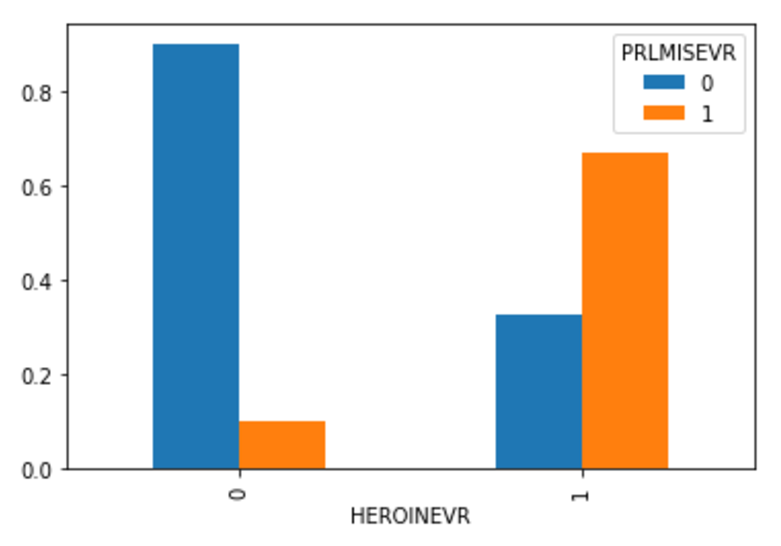
\includegraphics[width=\columnwidth]{images/Figure1.pdf}
  \caption{Proportion of Individuals Who Reported Ever Misusing Prescription
  Opioid Pain Relievers and Proportion Who Reported Using Heroin}
  \label{f:Figure1}
\end{figure}

%%%%%%%%%%%%%%%%%%%%%%%%%%%%%%%%%%%%%%%%%%%%%%%%%%%%%%%%%%%%%%%%%%%%%%%%%%%%%%%%
\subsection{Machine Learning Approaches} 

Machine learning is a set of procedures and automated processes for extracting 
knowledge from data. The two main branches of machine learning are' supervised 
learning and unsupervised learning. Supervised learning is used with problems 
that involve prediction about a specific target variable or outcome of interest. 
If a given dataset has no target outcome, unsupervised learning can be used to 
discover underlying structure in unlabeled data. The goal of this project is 
to classify opioid addiction and focuses on supervised learning. Supervised 
learning is used to predict a certain outcome from a given input, when examples 
of input/output pairs are available \cite{muller17}. A machine learning model 
is constructed from the training set of input-output pairs, to predict new test 
data not previously seen by the model. The two major approaches to supervised 
learning problems are regression and classification. When the target variable 
to be predicted is continuous, or there is continuity between the outcome 
(e.g., home values, or income), a regression model is used to test the set of 
features that predict the target variable. If the target is a class label, set 
of categorical or binary outcomes (e.g., `spam` or `ham`, `benign` or 
`malignant`), then classification is used to predict which class or category 
label that new instances will be assigned to.

\subsection{Classification Algorithms} 
Comparing the performance of different learning algorithms can be helpful for 
selecting the best model for a given problem \cite{raschka17}. One of the 
simplest classification algorithms is K-Nearest-Neighbors (KNN) which takes a 
set of data points and classifies a new data point based on the distance 
(Euclidean by default) to its nearest neighbor(s). The main parameter for KNN
is the number of neighbors, and typically k equal to 3 or 5 works well. KNN is
easy to understand and performs well with little adjustment, but it doe not 
perform well with datasets that have a large number of features (100 or more) 
or data that is sparse. For linear classification models, the decision boundary 
is a linear function of the input; a binary classifier separates two classes 
using along a line, plane, or hyperplane. Algorithms for linear classification 
differ in terms of (1) how they measure how well a particular combination of 
coefficients and intercept fit the training data, and (2) the type of 
regularization used \cite{muller17}. Two common linear classification models 
are logistic regression and support vector machines (SVMs). 


Decision Trees




%%%%%%%%%%%%%%%%%%%%%%%%%%%%%%%%%%%%%%%%%%%%%%%%%%%%%%%%%%%%%%%%%%%%%%%%%%%%%%%%
\subsection{Project Goals} 

The data for this project is the 2015 National Survey on Drug Use and Health 
(NSHUH-2015) \cite{samhsa16}. The NSDUH-2015 is a comprehensive survey that 
covers all aspects of substance use, misuse, dependency, and abuse, including 
questions related to both prescription medications (opioids, tranquilizers, 
sedatives) and illicit drugs (e.g., heroin, cocaine, methamphetamine), drug 
dependency, addiction, and treatment, demographic measures of education and 
employment, physical health, depression, and mental health treatment. The 
general idea of the project is that individuals dependent of addicted to 
prescription opioid medications are more likely to use illicit opioids such 
as heroin and fentanyl. Classifying individuals according to heroin use will 
identify the set of features the best predicts opioid addiction. Machine 
learning classification models were constructed to classify heroin use 
in the sample by demographics attributes and mental health characteristics 
(e.g., adult depression). This method helps address the opioid crisis in 
the following ways: (i) Identify factors related to opioid dependency and addiction, (ii) Inform consumers of prescription opioids about risk factors, 
and (iii) Increase knowledge about opioid abuse for better decisions by 
medication prescribers. 




%%%%%%%%%%%%%%%%%%%%%%%%%%%%%%%%%%%%%%%%%%%%%%%%%%%%%%%%%%%%%%%%%%%%%%%%%%%%%%%%
\section{Method}

\subsection{Data} 

Data from the 2015 NSHUH was downloaded from the Substance Abuse and Mental 
Health Data Archive (SAMHDA) \cite{samhsa16} URL using the `get-data.py` 
function written to unzip the data files, extract the data as a Pandas data 
frame, and write the file to CSV file \cite{getdata17}. The dataset consists 
of 57,146 observations with 2,666 features representing individual-level 
responses from a survey of the U.S. population. According to the NSDUH 
codebook, sampling was weighted across states by population size for a 
representative distribution selected from 6,000 area segments. The sample 
design used five state sample size groups drawing more heavily from the eight 
states with the largest population (e.g., CA, FL, IL, MI, NY, OH, PA, TX) which 
together account for 48 percent of total U.S. population aged 12 or older. 
All identifying information was collapsed (e.g., age categories) and state 
identifiers were removed from the public use file to ensure confidentiality. 
The NSDUH public-use files do not include geographic location, or demographic 
variables related to ethnicity or immigration status. The weighted survey 
screening response rate was 81.94 percent and the weighted interview response 
rate was 71.2 percent. 

%%%%%%%%%%%%%%%%%%%%%%%%%%%%%%%%%%%%%%%%%%%%%%%%%%%%%%%%%%%%%%%%%%%%%%%%%%%%%%%%
\subsection{Data Cleaning and Preparation }

\subsubsection{Data Cleaning}
All steps of this analysis was completed in a python interactive notebook 
\cite{data17} based following examples from \emph{Python for Data Analysis}
\cite{mckinney17}. After saving the NSDUH-2015 as a data frame object, the 
dataset was subset by columns to include demographic characteristics (e.g., 
age category, sex, marital status, education, employment status, and category 
of metropolitan area), measures of physical health (e.g., overall health, 
STDs, Hepatitis, HIV, Cancer, hospitalization), mental health (e.g., Adult 
Depression, Emotional Distress, Suicidal Thoughts, Plans), Suicide Attempts, 
Pain Reliever Medication Use, Misuse, and Abuse (over past year, past month), 
Prescription Opioid Medications Taken in Past year (e.g., Hydrocodone, 
Oxycodone, Tramadol, Morphine, Fentanyl,Oxymorphone, Demerol, Hydromorphone), 
Heroin Use, Abuse (over past year, past month), Tranquilizer Use, Sedative Use, 
Cocaine Use, Amphetamine and Methamphetamine Use, Hallucinogen Use, Drug 
Treatment (e.g., Inpatient, Outpatient, Hospital, Mental Health Clinic, ER, 
Drug Treatment Status), and Mental Health Treatment History. A codebook was 
created to provide a complete list of variables included with summaries 
of response categories \cite{codebook17}. Several steps to taken to detect 
and remove inconsistencies in the data \cite{rahm00}: 

\begin{enumerate}
  \item Missing values (i.e., `NaN`) were removed 
  \item Blanks, non-responses, or legitimate skips were recoded to zero 
  (e.g.,`99`, `991`, `993`) 
  \item Dichotomous responses (e.g., ``Yes=1``/``No=2``) were responses to 
  ``No=0``
  \item Categorical variables so the response was consistent with degree 
  (e.g., ``1=low``, ``2=med``, ``3=high``)
   \item Selected variables were renamed for better description (e.g., 
   Adult Major Depressive Episode Lifetime changed from `AMDELT` to `DEPMELT`)
\end{enumerate}

\subsubsection{Aggregate Variables}
Because the majority of features were represented as dichotomous ``Yes/No`` 
variables, related features were summed to create aggregated variables. For 
example, overall health, STD, Hepatitis, HIV, Cancer, and hospitalization were 
aggregated to create a single health measure. The health measure was recoded
so that higher scores indicated better health. Questions related to depression, 
emotional distress, and suicidal thoughts were summed to create a single 
variable for mental health (`MENTHLTH`) with scores ranging from 0 to 9. 
Responses to pain reliever medication use, misuse, abuse, or dependency, 
were aggregated to create a single variable of pain reliever misuse or abuse
(`PRLMISAB`). All prescription painkiller medications used in the past year
were summed. Similarly, all related responses were summed to create single 
variables for Tranquilizers, Sedatives, Cocaine, Amphetamines, Hallucinogens, 
Drug Treatment, and Mental Health Treatment. The target outcome of interest for 
classification, lifetime heroin use (i.e., ``Have you ever used heroin before, 
at any time?``) is a dichotomous variables. The demographic characteristics 
and aggregated variables were subset and saved to a new data frame consisting 
of 2` features and 57,146 observations, which was exported to CSV file. 


%%%%%%%%%%%%%%%%%%%%%%%%%%%%%%%%%%%%%%%%%%%%%%%%%%%%%%%%%%%%%%%%%%%%%%%%%%%%%%%%
\section{Results}

\subsection{Exploratory Analysis and Descriptives}\cite{mckinney17}

Of the total sample of N=57,146 respondents, 26,736 were male and 30,410 female;
6,343 individuals reported misusing pain medication at some point; however, 
only 956 repondents had used heroin at some point (570 males, 386 females). 




%Table\ref{t:mytable}. 

\begin{table}
  \caption{Substance Use by Age Group Counts - NSDUH 2015
  \cite{samhsa16}}
  \label{tab:freq}
  \begin{tabular}{cccccc}
    \toprule
    Age Group & 12-17& 18-25& 26-34& 35-49& 50+\\
    \midrule
    Sample Size & 13585& 14553& 9084& 11169& 8755 \\
    \midrule
    Oxycodone& 545& 1632& 1132& 1345& 1044 \\
    Hydrocodone& 831& 2936& 2233& 2781& 2103 \\
    Tramadol& 241& 753& 654& 829& 734 \\
    Morphine& 251& 431& 236& 313& 286 \\
    Fentanyl& 28& 97& 81& 96& 86 \\
    Demerol& 26& 74& 49& 64& 71 \\
    Buprenorphine& 43& 197& 167& 124& 51 \\
    Oxymorphone& 46& 88& 57& 47& 41 \\
    Hydromorphone& 24& 94& 107& 118& 81 \\
    \midrule
    PRL Misuse Ever*& 798& 2127& 1475& 1343& 600 \\
    \midrule
    Tranquilizers& 405& 1469& 1064& 1405& 1153 \\
    Sedatives& 204& 242& 157& 256& 226 \\
    Methadone Ever& 32& 83& 96& 71& 46&
    \midrule
    Heroin Use Ever*& 22& 261& 259& 250& 164 \\
    \midrule
    Cocaine Use Ever& 109& 1645& 1626& 1954& 1406 \\
    Amphetamines Ever& 932& 1836& 627& 383& 164&
    Methamphetamine& 42& 481& 700&  898& 492 \\
    Hallucinogens& 450& 2660& 2020& 2127& 1197 \\
    LSD Use Ever& 190& 1114& 874& 1442& 907 \\
    Exstasy (MDMA)& 199& 1867& 1403& 947& 149 \\
    \bottomrule
  \end{tabular}
\end{table}

Figure \ref{f:Figure2}, shows the aggregated measure of Opioid Pain Reliever 
misuse and abuse plotted against the aggregated measure of Heroin use (which
includes misuse, abuse, lifetime use, past year use, 30 day use), with
weighted regression lines by City Metropolitan region (from low to high). 
The highest proportions of opioid and heroin misuse and abuse is seen in 
large metropolitan areas with larger population size; however, the steeper
slope of the smaller metropolitan regions (e.g., Blue, Green points)
suggests that the highest levels of pain reliever abuse and misuse are
seen in smaller metropolitan and rural areas, but these are represented
by far fewer points. 

\begin{figure}[!ht]
  \centering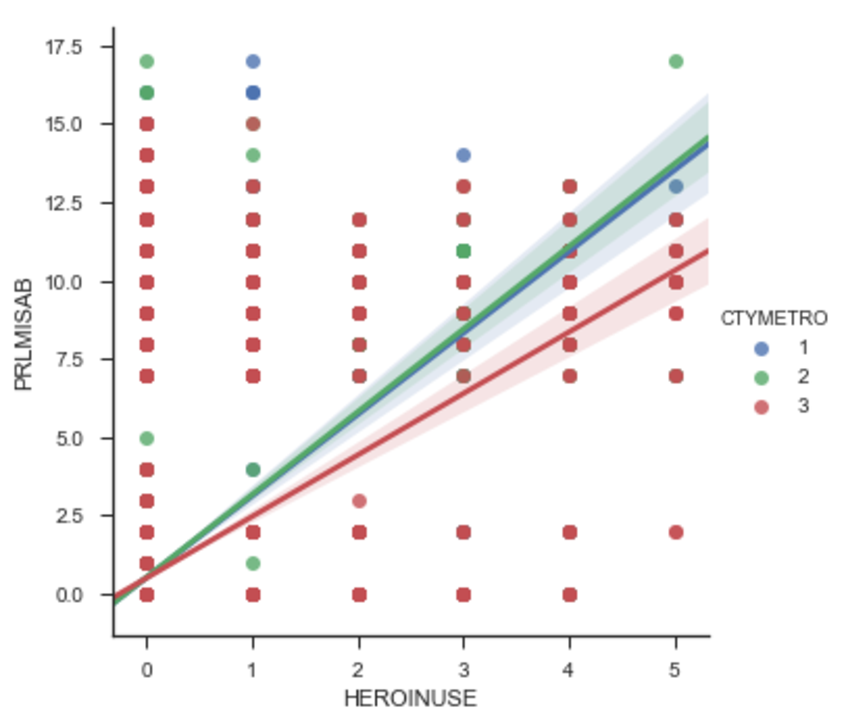
\includegraphics[width=\columnwidth]{images/Figure2.pdf}
  \caption{Plot of Opioid Pain Medication Misuse and Abuse and Heroin Use
  with Regression Slopes Weighted by Metropolitan Area Size}
  \label{f:Figure2}
\end{figure}


%%%%%%%%%%%%%%%%%%%%%%%%%%%%%%%%%%%%%%%%%%%%%%%%%%%%%%%%%%%%%%%%%%%%%%%%%%%%%%%%
\section{Classification Algorithms}

\cite{muller17}


\cite{raschka17}




\cite{vanderplas17}


%%%%%%%%%%%%%%%%%%%%%%%%%%%%%%%%%%%%%%%%%%%%%%%%%%%%%%%%%%%%%%%%%%%%%%%%%%%%%%%%
\section{Discussion}

\subsection{Extension to Big Data}

This classification method could be adopted for big data health analytics by
expanding the suvery to the popluation of patients with prescriptions for 
opioid pain medication and may help to identify individuals at risk for
potentially developing opioid dependency of addiction. 


Additional data from the NSDUH was downloaded from 2012 to 2014

hen trying to integrate data from multiple sources, (4) inconsistencies in coding of attributes or features can be a major source of problems. For example, time stamped data with different date formats (e.g., DD/MM/YY; YY/MM/DD, or MM/DD/YY) would have to be reformatted before being combined. Similarly, different coding for sex (e.g., ‘M’/’F’, ‘0’/’1’, ‘1’,’2’) have to be reconciled when combining multiple data sources. Cleaning big data is a more involved process, with Extraction, Integration, and Aggregation of data from operationalized sources into a data warehouse. In general, there are several phases involved in big data cleaning approaches, including the following:

%%%%%%%%%%%%%%%%%%%%%%%%%%%%%%%%%%%%%%%%%%%%%%%%%%%%%%%%%%%%%%%%%%%%%%%%%%%%%%%%
\subsection{Limitations}

Tradeoff between quality and quantity


To be of any use, diverse and often messy raw data has to be sifted through and 
effectively organized for further analysis, and 


there are legitimate questions about the reliability of self report data from survey
research for predicting actual behavior. 

The question of 
Value evaluates the quality of the data as it pertains to intended outcomes, such 
as limiting the spread of contagion and disease prevention. 

An important challenge for making sense of big data is developing analytic 
tools adequate to handle large volumes of data in real time.

%%%%%%%%%%%%%%%%%%%%%%%%%%%%%%%%%%%%%%%%%%%%%%%%%%%%%%%%%%%%%%%%%%%%%%%%%%%%%%%%
\subsection{Drug Abuse, Dependency, and Addiction}

Drug addiction has many similar characteristics to other chronic medical 
illnesses, but there are unique challenges to the treatment of addiction
\cite{marsch12, swendson16}. In drug rehabilitation treatment programs, 
patients undergo intense detoxification that reduces their drug tolerance, but 
are then released back into the environments associated with their drug use, 
putting them at high risk for relapse and potential drug overdose 
\cite{johnson11}. According to a classical conditioning model of addiction, 
situational cues or events can elicit a motivational state underlying relapse 
to drug use. Addictive behavior can be also be reinstated after extinction of 
dependency by exposure to drug-related cues or stressors in the environment 
\cite{shaham03}. 


%%%%%%%%%%%%%%%%%%%%%%%%%%%%%%%%%%%%%%%%%%%%%%%%%%%%%%%%%%%%%%%%%%%%%%%%%%%%%%%%
\subsection{Dynamics of Epidemic Spreading}

Epidemic spreading is a complex phenomenon based on contact networks between 
individuals and distributed by transportation networks \cite{Colizza06}.

The dynamics of epidemic spreading is a complex phenomenon, based on contact 
networks of person-to-person interaction, indirect exposure, and transmission 
byways such as the {\it airline transportation network} (ATN) \cite{Colizza06}. 
Epidemics are quantified in terms of the proportion of the population infected, 
those yet to be infected, and the rate of transmission \cite{hethcote00}. In 
addition, the structure of the contact network can influence epidemic spreading 
\cite{pastor01}. For example, in the case of simple contagion, weak ties among 
acquaintances or infrequent associations provide shortcuts between distant nodes 
that reduce distance within the network \cite{granovetter73} and can facilitate 
the spread of disease. 

Furthermore, networks with ``small world'' properties have many nodes with 
few connections, but a small number of highly connected nodes that can rapidly 
transmit contagion throughout the network \cite{watts98}. Analyzing the 
correlation between Twitter posts and rate of ILI reports does not capture the 
complex network structure that underlies disease epidemics and pandemics. 
It is possible that by analyzing the structure of social media networks, 

future research may help to identify how points of connection within online
networks are associated with the spread of contagion and resulting epidemics 
\cite{zhu17}. Some epidemics such as the opioid crisis in North America 
\cite{volkow14} may be amenable to social network modeling as drug usage, 
dependancy, and addiction is subserved by social networks. The emergence of 
new technologies, such as wearable biosensors \cite{carreiro15} may help 
improve geospatial mapping of the opioid epidemics and treatment interventions.

%%%%%%%%%%%%%%%%%%%%%%%%%%%%%%%%%%%%%%%%%%%%%%%%%%%%%%%%%%%%%%%%%%%%%%%%%%%%%%%%
\section{Conclusion}

Machine learning classification of opioid abuse can contribute to efforts to address prescription opioid addiction, overdoses, in the following ways: 
\begin{enumerate}
\item Identify factors related to opioid dependency
\item Inform consumers of opioid medication as to risk factors 
\item Increase knowledge of opioid abuse for more informed prescriptions. 
\end{enumerate}


%%%%%%%%%%%%%%%%%%%%%%%%%%%%%%%%%%%%%%%%%%%%%%%%%%%%%%%%%%%%%%%%%%%%%%%%%%%%%%%%

\section{figures}




%%%%%%%%%%%%%%%%%%%%%%%%%%%%%%%%%%%%%%%%%%%%%%%%%%%%%%%%%%%%%%%%%%%%%%%%%%%%%%%%
\section{Tables}

%Table\ref{t:mytable}. 

\begin{table}
  \caption{Frequency Table of Mental Health Issues and Treatment NSDUH 2015
  \cite{samhsa16}}
  \label{tab:freq}
  \begin{tabular}{cccccc}
    \toprule
    Age Group & 12-17& 18-25& 26-34& 35-49& 50+\\
    \midrule
    In Hospital Overnight& 730& 1149& 821& 890& 1173 \\
    Adult Depression& 0& 2413& 1395& 1766& 967 \\
    Suicidal Thoughts& 13585& 14553& 9084& 11189& 8755 \\
    \midrule
    Mental Health Treatment& & & & & \\
    \midrule
    Private Therapist& 0& 592& 434& 554& 311 \\
    Treatment Gap*& 469& 931& 321& 239& 90 \\
    \bottomrule
  \end{tabular}
\end{table}



%%%%%%%%%%%%%%%%%%%%%%%%%%%%%%%%%%%%%%%%%%%%%%%%%%%%%%%%%%%%%%%%%%%%%%%%%%%%%%%%
\begin{acks}

  The author would like to thank Dr. Gregor von Laszewski, 
  the Assistant Instructors, Juliette Zurick, Miao Zheng,
  and others who helped to improve this project and report.

\end{acks}

\bibliographystyle{ACM-Reference-Format}
\bibliography{report} 


%%%%%%%%%%%%%%%%%%%%%%%%%%%%%%%%%%%%%%%%%%%%%%%%%%%%%%%%%%%%%%%%%%%%%%%%%%%%%%%%
\appendix



\section{Code References}

All code, notebooks, files, and folders for this project can be found in the
project githup repository: \url{url:  https://github.com/bigdata-i523/hid335/tree/master/project}.

\subsection{Download and Extract Data file \cite{getdata17}}

The `get-data.py` function was written to download the data, unzip the data
files, extract the data, and write the NSDUH-2015 dataset to CSV file 
\cite{getdata17}.

\subsection{Data Cleaning and Preparation \cite{mckinney17}}

Data cleaning and preparation steps was conducted based on examples in 
Chapter 7 of Python for Data Analysis \cite{mckinney17} and Chapter 3 in 
the Python Data Science Handbook \cite{vanderplas17}, using an interactive 
python Jupyter Notebook: \url{url: https://github.com/bigdata-i523/hid335/blob/master/project/BDA_Project_Data.ipynb}.

\subsection{Exploratory Data Analysis and Visualization\cite{vanderplas17}}

Exploratory Data Analysis and Visualization was based on examples included
in Python for Data Analysis \cite{mckinney17}, and the Python Data Science 
Handbook \cite{vanderplas17}, and were executed in the following interative
python notebook: 


\subsection{Machine Learning Classification Algorithms\cite{muller17, raschka17}}
Machine Learning Classification algorithms were based on examples provided
in Chapters 2 and 5 of an Introduction to Machine Learning \cite{muller17},
and Chapters 3 and 4 in Python Machine Learning \cite{raschka17}. All 
classification models were constructed in an interative python notebook: 


%\begin{enumerate}

%\item Do not to use the underscore in bibtex labels
%\item Address each of the items in the issues.tex file  and verify you have done them. 
%item Please do this only at the end once you have finished writing the paper. 
%\item Change `TODO` with `DONE`. 

%\end{enumerate}

%\section{Issues}

\DONE{Example of done item: Once you fix an item, change TODO to DONE}

\subsection{Assignment Submission Issues}

    \DONE{Do not make changes to your paper during grading, when your repository should be frozen.}

\subsection{Uncaught Bibliography Errors}

    \DONE{Missing bibliography file generated by JabRef}
    \DONE{Bibtex labels cannot have any spaces, \_ or \& in it}
    \DONE{Citations in text showing as [?]: this means either your report.bib is not up-to-date or there is a spelling error in the label of the item you want to cite, either in report.bib or in report.tex}

\subsection{Formatting}

    \DONE{Incorrect number of keywords or HID and i523 not included in the keywords}
    \DONE{Other formatting issues}

\subsection{Writing Errors}

    \DONE{Errors in title, e.g. capitalization}
    \DONE{Spelling errors}
    \DONE{Are you using {\em a} and {\em the} properly?}
    \DONE{Do not use phrases such as {\em shown in the Figure below}. Instead, use {\em as shown in Figure 3}, when referring to the 3rd figure}
    \DONE{Do not use the word {\em I} instead use {\em we} even if you are the sole author}
    \DONE{Do not use the phrase {\em In this paper/report we show} instead use {\em We show}. It is not important if this is a paper or a report and does not need to be mentioned}
    \DONE{If you want to say {\em and} do not use {\em \&} but use the word {\em and}}
    \DONE{Use a space after . , : }
    \DONE{When using a section command, the section title is not written in all-caps as format does this for you}\begin{verbatim}\section{Introduction} and NOT \section{INTRODUCTION} \end{verbatim}

\subsection{Citation Issues and Plagiarism}

    \DONE{It is your responsibility to make sure no plagiarism occurs. The instructions and resources were given in the class}
    \DONE{Claims made without citations provided}
    \DONE{Need to paraphrase long quotations (whole sentences or longer)}
    \DONE{Need to quote directly cited material}

\subsection{Character Errors}

    \DONE{Erroneous use of quotation marks, i.e. use ``quotes'' , instead of " "}
    \DONE{To emphasize a word, use {\em emphasize} and not ``quote''}
    \DONE{When using the characters \& \# \% \_  put a backslash before them so that they show up correctly}
    \DONE{Pasting and copying from the Web often results in non-ASCII characters to be used in your text, please remove them and replace accordingly. This is the case for quotes, dashes and all the other special characters.}
    \DONE{If you see a figure and not a figure in text you copied from a text that has the fi combined as a single character}

\subsection{Structural Issues}

    \DONE{Acknowledgement section missing}
    \DONE{Incorrect README file}
    \DONE{In case of a class and if you do a multi-author paper, you need to add an appendix describing who did what in the paper}
    \DONE{The paper has less than 2 pages of text, i.e. excluding images, tables and figures}
    \DONE{The paper has more than 6 pages of text, i.e. excluding images, tables and figures}
    \DONE{Do not artificially inflate your paper if you are below the page limit}

\subsection{Details about the Figures and Tables}

    \DONE{Capitalization errors in referring to captions, e.g. Figure 1, Table 2}
    \DONE{Do use {\em label} and {\em ref} to automatically create figure numbers}
    \DONE{Wrong placement of figure caption. They should be on the bottom of the figure}
    \DONE{Wrong placement of table caption. They should be on the top of the table}
    \DONE{Images submitted incorrectly. They should be in native format, e.g. .graffle, .pptx, .png, .jpg}
    \DONE{Do not submit eps images. Instead, convert them to PDF}

    \DONE{The image files must be in a single directory named "images"}
    \DONE{In case there is a powerpoint in the submission, the image must be exported as PDF}
    \DONE{Make the figures large enough so we can read the details. If needed make the figure over two columns}
    \DONE{Do not worry about the figure placement if they are at a different location than you think. Figures are allowed to float. For this class, you should place all figures at the end of the report.}
    \DONE{In case you copied a figure from another paper you need to ask for copyright permission. In case of a class paper, you must include a reference to the original in the caption}
    \DONE{Remove any figure that is not referred to explicitly in the text (As shown in Figure ..)}
    \DONE{Do not use textwidth as a parameter for includegraphics}
    \DONE{Figures should be reasonably sized and often you just need to
  add columnwidth} e.g. \begin{verbatim}/includegraphics[width=\columnwidth]{images/myimage.pdf}\end{verbatim}

re


\end{document}
